\documentclass{ieeeaccess}
\usepackage{cite}
\usepackage{amsmath,amssymb,amsfonts}
\usepackage{algorithmic}
\usepackage{algorithm}
\usepackage{graphicx}
\usepackage{textcomp}
\usepackage{booktabs}
\usepackage{xcolor}
\usepackage{tikz}
\usetikzlibrary{arrows.meta,positioning}
\def\BibTeX{{\rm B\kern-.05em{\sc i\kern-.025em b}\kern-.08em
    T\kern-.1667em\lower.7ex\hbox{E}\kern-.125emX}}
\newcommand{\bphi}{\boldsymbol{\phi}}
\newcommand{\bw}{\mathbf{w}}
\begin{document}
\history{Date of publication xxxx 00, 0000, date of current version xxxx 00, 0000.}
\doi{10.1109/ACCESS.2025.DOI}

\title{Interpretable Maximum Entropy Inverse Reinforcement Learning for Route Preference Learning on Porto Taxi GPS Data}
\author{\uppercase{Abhinav Nair}\authorrefmark{1},
\uppercase{Advaith K}\authorrefmark{1}, and
\uppercase{Akash A}\authorrefmark{1}}
\address[1]{Department of Computer Science Engineering (Artificial Intelligence), Amrita Vishwa Vidyapeetham, Amritapuri, India}
\tfootnote{This work was carried out for the course 22AIE401 Reinforcement Learning (Phase 2 report) at Amrita Vishwa Vidyapeetham, Amritapuri.}

\markboth
{Nair \headeretal: Interpretable MaxEnt IRL for Route Preference Learning}
{Nair \headeretal: Interpretable MaxEnt IRL for Route Preference Learning}

\corresp{Corresponding author: Abhinav Nair (e-mail: abhinavnair2nt5@gmail.com).}

\begin{abstract}
Drivers rarely take the shortest or fastest route, and the preferences behind their choices are never observed directly. We learn these preferences with Maximum Entropy Inverse Reinforcement Learning (MaxEnt IRL) on the central Porto road network, using map-matched GPS trips from the ECML/PKDD 2015 taxi dataset. The network is modelled as a goal-conditioned, deterministic-transition Markov Decision Process with a reward that is linear in interpretable road, turn and familiarity features. Road and turn features alone only match Dijkstra's shortest path on route overlap (Jaccard 0.52 vs.\ 0.54). Our main contribution is a data-driven edge-familiarity feature, which raises held-out log-likelihood per step from $-0.179$ to $-0.158$ and yields Jaccard 0.57--0.59 under 5-fold cross-validation, above shortest path (0.538). A non-learned popularity-weighted shortest path remains slightly ahead on overlap (0.594). Time-of-day context conditioning gave no measurable gain.
\end{abstract}

\begin{keywords}
Inverse reinforcement learning, interpretability, Markov decision process, maximum entropy, route choice, taxi GPS
\end{keywords}


\titlepgskip=-15pt

\maketitle

\section{Introduction}
\PARstart{N}{avigation} systems route by distance, time and traffic, but drivers also weigh road quality, turn difficulty and habit. Inverse Reinforcement Learning (IRL) reverses the usual RL setting: it infers the reward that makes observed behaviour (near-)optimal~\cite{ziebart2008maxent}. A reward that is linear in named features can be read directly and used to generate human-aligned routes.

\textbf{Research gap.} Static routing ignores subjective trade-offs, supervised predictors are black boxes, and existing IRL route systems are computationally heavy, proprietary or hard to reproduce (Section~\ref{sec:related}).

\textbf{Objective.} Learn interpretable driver route preferences from historical GPS trajectories on an OpenStreetMap (OSM) network, and generate realistic routes for unseen origin--destination (OD) pairs.

\textbf{Contributions.}
(1)~A reproducible open-data pipeline from raw GPS to an exact MaxEnt IRL trainer.
(2)~An identifiable, interpretable feature set and explicit MDP formulation.
(3)~A data-driven \emph{edge-familiarity} feature, the main positive result.
(4)~A statistically careful evaluation (bootstrap CIs, paired tests, cross-validation) that reports negative results.

%--------------------------------------------------------------
\section{Related Work}\label{sec:related}
\begin{table}[t]
\centering\footnotesize
\caption{Related work and limitations relative to this project.}\label{tab:related}
\begin{tabular}{@{}p{1.9cm}p{2.5cm}p{3.1cm}@{}}
\toprule
Work & Method & Limitation / gap\\
\midrule
Ziebart '08~\cite{ziebart2008maxent} & MaxEnt IRL & Small-scale, hand features; no modern open-data study\\
Ziebart '08~\cite{ziebart2008cabbie} & Context-aware taxi route prediction & Pittsburgh data not public; no ablation of familiarity\\
Fosgerau '13~\cite{fosgerau2013} & Recursive logit & Equivalent to soft DP; no IRL/RL evaluation\\
Liu '20~\cite{liu2020} & Deep IRL + Dijkstra (delivery) & Black-box reward\\
Zhao \& Liang '23~\cite{zhao2023} & Deep context-dependent IRL & Not interpretable; heavy\\
Barnes '24~\cite{barnes2024} & IRL at Google Maps scale & Proprietary data/model; irreproducible\\
Zhang '24~\cite{zhang2024} & Recursive-logit meta-IRL & Complex; efficiency-focused\\
Pitombeira-Neto '24~\cite{pitombeira2024} & Random-utility IRL & Statistical focus, no route-overlap benchmark\\
\bottomrule
\end{tabular}
\end{table}
Table~\ref{tab:related} shows that open, exact and interpretable IRL with an explicit baseline comparison on public data is under-served. We do not claim novelty for the algorithm itself; our angle is the interpretable linear reward, the familiarity feature, and a transparent evaluation.

%--------------------------------------------------------------
\section{Problem Formulation}\label{sec:problem}
The task is a fully observable, goal-conditioned MDP $\mathcal M=\langle S,A,P,R,\gamma\rangle$ whose reward is unknown (Fig.~\ref{fig:mdp}).

\Figure[t!](topskip=0pt, botskip=0pt, midskip=0pt)[width=0.98\columnwidth]{figures/mdp_full.png}
{MDP structure and linear reward $R(s,a)=\bw^\top\bphi(s,a)$ (original 10-feature set; final features in Table~\ref{tab:feat}).\label{fig:mdp}}

\textbf{State.} $s_t=e_{t-1}=(u\!\rightarrow\! v)$, the directed edge just traversed. A node alone loses the heading needed for turn angles; full history is needlessly large. The incoming edge makes the process Markov. The destination $d$ is a fixed episode parameter.

\textbf{Action.} $A(e)=\{e':\mathrm{tail}(e')=\mathrm{head}(e)\}$, typically 2--4 outgoing roads. U-turns are allowed but penalised.

\textbf{Transition.} Deterministic: $P(s'{=}a\mid s,a)=1$. Randomness lives in the driver's policy.

\textbf{Reward.} $R(s,a)=\bw^\top\bphi(s,a)$, unknown. Turn features depend on $(s,a)$, which is why the state carries the heading.

\textbf{Constraints and horizon.} Moves must follow the directed road graph. The task is episodic with $\gamma=1$; the destination is absorbing ($V=0$); soft values use horizon $H=80$, matching the 5--75-edge trip filter.

\textbf{Objective.} Given demonstrations $\mathcal D=\{(\xi_i,d_i)\}$, find
\begin{equation}
\bw^\star=\arg\max_{\bw}\ \sum_i \log P(\xi_i\mid\bw,d_i)-\tfrac{\lambda}{2}\|\bw\|^2,
\end{equation}
where $P(\xi|\bw,d)=\exp(\bw^\top\mathbf f(\xi))/Z$ and $\mathbf f(\xi)=\sum_t\bphi(s_t,a_t)$.

\textbf{Soft policy.}
\begin{align}
Q(e,e') &= \bw^\top\bphi(e,e')+V(e'),\\
V(e) &= \log\textstyle\sum_{e'}\exp Q(e,e'),\quad \pi(e'|e)=e^{Q(e,e')-V(e)}.
\end{align}

\textbf{Assumptions.} One reward for all drivers and times; map-matched GPS treated as truth; destination known; no congestion dynamics.

%--------------------------------------------------------------
\section{Proposed Methodology}\label{sec:method}
\subsection{Learning the reward}
The gradient of the objective is
\begin{equation}
\nabla_{\bw}\mathcal L=\tilde{\mathbf f}-\mathbb E_{\pi_{\bw}}[\mathbf f]-\lambda\bw,
\end{equation}
expert feature counts minus expected counts under the current soft policy. Algorithm~\ref{alg:irl} gives the full procedure.

\begin{algorithm}[t]
\caption{MaxEnt IRL on the road graph}\label{alg:irl}
\begin{algorithmic}[1]
\REQUIRE graph $G$, trips $\mathcal D$, features $\bphi$, horizon $H$, $\lambda$
\STATE $\tilde{\mathbf f}\gets\frac1{|\mathcal D|}\sum_i \mathbf f(\xi_i)$; initialise $\bw$
\REPEAT \COMMENT{L-BFGS outer loop}
  \FOR{each destination $d$ (in parallel)}
    \STATE \textbf{backward:} $V_d(e)\gets\log\sum_{e'}\exp(\bw^\top\bphi+V_d(e'))$ for $H$ levels, $V_d=0$ at $d$
    \STATE $\pi_d(e'|e)\gets\exp(Q_d-V_d)$
    \STATE \textbf{forward:} propagate origin mass through $\pi_d$ to get visitation $\rho_d$
    \STATE $\mathbb E_{\pi}[\mathbf f]_d\gets\sum_{e,e'}\rho_d(e)\pi_d(e'|e)\bphi(e,e')$
  \ENDFOR
  \STATE $\nabla\gets\tilde{\mathbf f}-\mathbb E_\pi[\mathbf f]-\lambda\bw$; update $\bw$ with L-BFGS
\UNTIL{converged or 35 iterations}
\STATE \textbf{Prediction:} route $\hat\xi=$ shortest path on cost $-\bw^\top\bphi$ (plus validation-chosen length offset $\alpha$)
\end{algorithmic}
\end{algorithm}


\subsection{Novel elements}
(i)~An identifiable feature set (Table~\ref{tab:feat}) fixing the collinearity of a naive set; (ii)~a leakage-free \emph{edge familiarity} feature $\log(1{+}n_e)/\log(1{+}n_{\max})$ from an independent trip pool; (iii)~validation-only decision-time calibration; (iv)~an exact, finite-difference-verified implementation (max relative gradient error $1.3\times10^{-7}$).

\begin{table}[t]
\centering\footnotesize
\caption{Feature sets.}\label{tab:feat}
\begin{tabular}{@{}p{0.8cm}p{4.9cm}p{2cm}@{}}
\toprule
Set & Features & Note\\
\midrule
v1 & length, speed, time, 3 road classes, 3 turn types, lanes & collinear (corr 0.81)\\
v2 & length, time, step, motorway, primary, slight/sharp turn, lanes, same road name, away-from-goal & identifiable\\
v3 & v2 + edge familiarity & independent pool\\
\bottomrule
\end{tabular}
\end{table}
A signed progress-to-goal term was rejected: it telescopes to a per-trip constant and cancels in MaxEnt IRL, so the indicator \texttt{away\_from\_goal} is used.

%--------------------------------------------------------------
\section{System and Model Design}\label{sec:system}
\begin{figure}[t]
\centering
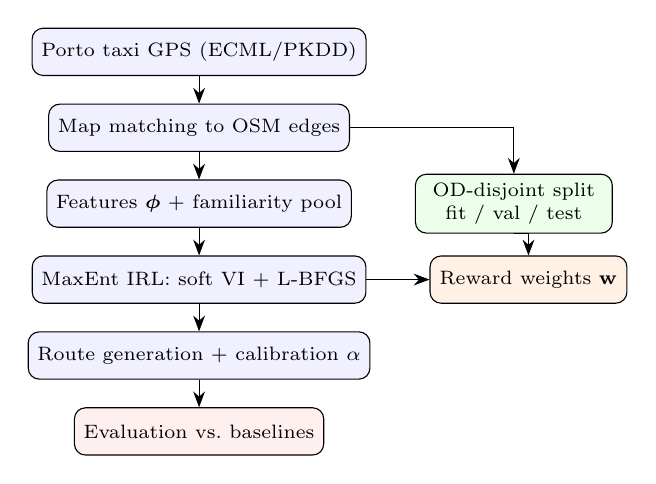
\begin{tikzpicture}[node distance=3.5mm, every node/.style={font=\scriptsize},
  box/.style={draw,rounded corners,align=center,minimum width=2.5cm,minimum height=6mm,fill=blue!6},
  arr/.style={-{Stealth[length=2mm]}}]
\node[box] (a){Porto taxi GPS (ECML/PKDD)};
\node[box,below=of a] (b){Map matching to OSM edges};
\node[box,below=of b] (c){Features $\bphi$ + familiarity pool};
\node[box,below=of c] (d){MaxEnt IRL: soft VI + L-BFGS};
\node[box,right=8mm of c,fill=green!8] (e){OD-disjoint split\\fit / val / test};
\node[box,right=8mm of d,fill=orange!10] (f){Reward weights $\bw$};
\node[box,below=of d] (g){Route generation + calibration $\alpha$};
\node[box,below=of g,fill=red!6] (h){Evaluation vs.\ baselines};
\draw[arr](a)--(b);\draw[arr](b)--(c);\draw[arr](c)--(d);
\draw[arr](b.east)-|(e.north);\draw[arr](e.south)--(f.north|-e.south)--(f.north);
\draw[arr](d)--(f);\draw[arr](d)--(g);\draw[arr](g)--(h);
\end{tikzpicture}
\caption{System workflow from raw GPS to evaluation.}\label{fig:flow}
\end{figure}
Fig.~\ref{fig:flow} shows the pipeline; modules and interfaces are in Table~\ref{tab:modules}.

\begin{table}[t]
\centering\footnotesize
\caption{Modules (code in \texttt{src/}).}\label{tab:modules}
\begin{tabular}{@{}p{1.6cm}p{2.9cm}p{2.9cm}@{}}
\toprule
Module & Input & Output\\
\midrule
Map matcher & GPS points, OSM graph & edge sequence per trip\\
Feature builder & graph, familiarity pool & $\bphi(e,e')$ matrix\\
\texttt{mdp.py} & $\bw$, destination & soft $V,Q,\pi$; best route\\
\texttt{maxent\_irl.py} & trips, features & learned $\bw$\\
\texttt{evaluation.py} & routes, ground truth & overlap, LL, accuracy, CIs\\
\bottomrule
\end{tabular}
\end{table}

%--------------------------------------------------------------
\section{Experimental Setup}\label{sec:setup}
\textbf{Data.} Taxi Service Trajectory data (442 taxis, 1.71M trips)~\cite{moreira2013,porto2015} in a central Porto box ($41.14$--$41.185^\circ$N, $-8.65$ to $-8.58^\circ$E). OSMnx \texttt{drive} graph: 3{,}367 nodes, 6{,}784 directed edges. 56\% of trips map-matched (median route/GPS length ratio 1.09); trips of 5--75 edges kept.

\textbf{Splits.} OD-disjoint: 2{,}040 fit / 360 validation / 600 test trips. A separate 3{,}000-trip pool (disjoint by trip id) builds the familiarity feature. Cross-validation uses 5 folds.

\textbf{Baselines.} Dijkstra-shortest; Dijkstra-fastest; myopic logistic-regression classifier; popularity-weighted shortest path (Pop-Shortest, cost $=$ length / familiarity); and an \emph{RL planner with a hand-designed reward} (RL-Handcrafted): the same soft value iteration and route extraction as our method but a fixed reward ($-1$ per 100\,m, $-1$ sharp turn, $-0.3$ slight turn) that is not learned from data.

\textbf{Hyperparameters.} $L_2$ weight $\lambda=10^{-3}$; horizon $H=80$; 35 L-BFGS iterations, warm-started from v2 for v3; length offset $\alpha$ chosen on validation ($\alpha=1.0$ for v2, $0.5$ for v3); context shrinkage $0.5$.

\textbf{Hardware/cost.} Training is parallelised over destinations (7 workers), about 20 min per fit. A synthetic San Francisco run is the correctness check (weight-recovery cosine similarity 0.987).

\textbf{Statistics.} 95\% bootstrap CIs over trips; paired Wilcoxon tests on identical trips; mean $\pm$ std over folds.

%--------------------------------------------------------------
\section{Performance Evaluation Metrics}\label{sec:metrics}
\textbf{Problem-specific (route quality).} Edge Jaccard and F1 between generated and recorded route; path-length ratio $=$ generated / recorded length.

\textbf{Policy/RL-specific.} Held-out log-likelihood per step and trip NLL, i.e.\ how probable the driver's actions are under the learned soft policy (the IRL objective on unseen data); top-1/top-3 next-edge accuracy, i.e.\ agreement between the policy's greedy action and the driver's action at each junction.

\textbf{Geometric.} Discrete Fr\'echet distance (metres, lower is better) between the predicted and recorded node polylines.

\textbf{Not reported.} Expected value difference needs a ground-truth reward, which exists only for the synthetic San Francisco run, so it is not defined for real Porto data.

%--------------------------------------------------------------
\section{Results and Discussion}\label{sec:results}
\subsection{Initial MaxEnt IRL (v1)}
\begin{table}[t]
\centering\footnotesize
\caption{Initial results, 600 test trips (Jaccard with 95\% CI).}\label{tab:v1}
\begin{tabular}{@{}lccc@{}}
\toprule
Method & Jaccard & F1 & Len.\ ratio\\
\midrule
Dijkstra-Shortest & 0.541 [.514,.568] & 0.636 & 0.884\\
Dijkstra-Fastest & 0.357 [.334,.383] & 0.454 & 1.011\\
Myopic classifier & 0.059 [.049,.070] & -- & --\\
MaxEnt IRL (v1) & 0.521 [.493,.549] & 0.611 & 0.924\\
\bottomrule
\end{tabular}
\end{table}
IRL strongly beats the myopic classifier and fastest path, but is tied with shortest path on Jaccard ($p=0.12$) and slightly worse on F1 ($p=0.029$). Top-1/top-3 accuracy is 0.927/0.999; LL is $-0.174$ per step. \emph{Why:} drivers' routes are 15.6\% longer than the shortest path, IRL and shortest path agree on only 44\% of trips, and v1's collinear features give uninterpretable weights.

\subsection{Learned reward}
\Figure[t!](topskip=0pt, botskip=0pt, midskip=0pt)[width=0.98\columnwidth]{figures/weights_v3.png}
{Learned v3 weights. Sharp turns are most penalised; familiarity is the only large positive weight. Length and time are correlated (0.81): read them jointly.\label{fig:w}}
Drivers strongly avoid sharp turns and moving away from the goal, and favour roads that other taxis commonly use.

\subsection{Convergence}
\Figure[t!](topskip=0pt, botskip=0pt, midskip=0pt)[width=0.95\columnwidth]{figures/cv_training_curves.png}
{Training NLL per trajectory (mean $\pm$ std over folds). Both feature sets converge within about 10 iterations; v3 settles lower (about 5.7 vs.\ 6.3).\label{fig:conv}}

%--------------------------------------------------------------
\section{Comparison with Benchmark Methods}\label{sec:compare}
\begin{table*}[t]
\centering\footnotesize
\caption{5-fold cross-validation, mean $\pm$ std over folds (seed 0). Fr\'echet is not computed for v2 (no stored routes). Raw and calibrated IRL share likelihood because calibration only changes route extraction.}\label{tab:cv}
\begin{tabular}{lcccccc}
\toprule
Method & Jaccard & F1 & Len.\ ratio & Fr\'echet (m) & LL / step & Trip NLL\\
\midrule
Dijkstra-Fastest & $0.378\pm0.009$ & $0.476\pm0.010$ & $1.009\pm0.007$ & $519.6\pm12.8$ & -- & --\\
Dijkstra-Shortest & $0.539\pm0.003$ & $0.630\pm0.002$ & $0.884\pm0.005$ & $367.5\pm7.1$ & -- & --\
RL-Handcrafted (fixed reward) & $0.545\pm0.009$ & $0.636\pm0.008$ & $0.890\pm0.005$ & $365.3\pm7.8$ & -- & --\\
Pop-Shortest & $\mathbf{0.594\pm0.005}$ & $\mathbf{0.671\pm0.006}$ & $0.903\pm0.010$ & $354.7\pm6.6$ & -- & --\\
IRL-v2 (raw) & $0.530\pm0.013$ & $0.617\pm0.007$ & $0.916\pm0.002$ & -- & $-0.179\pm0.007$ & $6.15\pm0.46$\\
IRL-v2 (calibrated) & $0.563\pm0.007$ & $0.650\pm0.005$ & $0.885\pm0.002$ & -- & $-0.179\pm0.007$ & $6.15\pm0.46$\\
IRL-v3 (raw) & $0.572\pm0.009$ & $0.655\pm0.007$ & $0.929\pm0.007$ & $369.6\pm10.0$ & $\mathbf{-0.158\pm0.005}$ & $\mathbf{5.50\pm0.26}$\\
IRL-v3 (calibrated) & $0.588\pm0.010$ & $0.669\pm0.009$ & $0.899\pm0.007$ & $\mathbf{348.3\pm16.2}$ & $\mathbf{-0.158\pm0.005}$ & $\mathbf{5.50\pm0.26}$\\
\bottomrule
\end{tabular}
\end{table*}

\Figure[t!](topskip=0pt, botskip=0pt, midskip=0pt)[width=0.85\textwidth]{figures/cv_methods_bars.png}
{Cross-validated comparison of all methods (mean $\pm$ std over folds).\label{fig:cv}}

Table~\ref{tab:cv} compares IRL with classical routing (Dijkstra), a supervised learner (myopic classifier) and a strong non-learned popularity baseline. IRL-v3 has the best likelihood (about 12\% better than v2 per step) and beats plain shortest path on overlap (0.572--0.588 vs.\ 0.538). However, Pop-Shortest is slightly ahead on overlap (0.594), so a simple non-learned use of the familiarity signal is hard to beat; IRL's advantage is a calibrated probabilistic model and interpretable weights. The single-split calibrated v3 figure (0.601) exceeds the cross-validated mean (0.588), and the latter should be quoted.

\textbf{RL vs.\ IRL.} RL-Handcrafted is the planner one would write without data (Jaccard $0.545$, Fr\'echet $365$\,m). Learning the reward from demonstrations improves overlap to $0.572$--$0.588$ and, after calibration, gives the lowest Fr\'echet of all methods ($348$\,m, though within about one standard deviation of Pop-Shortest at $355$\,m).

\textbf{Scope of comparison.} We did not reimplement deep-RL or published IRL systems~\cite{zhao2023,barnes2024,liu2020}; they use different data, so published numbers are not directly comparable. A deep-RL or adversarial-IRL baseline is not included.

%--------------------------------------------------------------
\section{Ablation Study}\label{sec:ablation}
\begin{table}[t]
\centering\footnotesize
\caption{Single-split ablation, 600 test trips ($p$ vs.\ Dijkstra-shortest).}\label{tab:abl}
\begin{tabular}{@{}lcccc@{}}
\toprule
Variant & Jaccard & F1 & LL/step & $p$\\
\midrule
Dijkstra-Shortest & 0.541 & 0.636 & -- & --\\
v1 (collinear features) & 0.521 & 0.611 & $-.174$ & 0.12\\
v2 (identifiable) & 0.519 & 0.606 & $-.173$ & 0.086\\
v2 + calibration & 0.563 & 0.648 & $-.173$ & 0.017\\
v3 (+ familiarity) & 0.578 & 0.659 & $-.155$ & 0.009\\
v3 + calibration & \textbf{0.601} & \textbf{0.682} & $-.155$ & $6{\times}10^{-7}$\\
\bottomrule
\end{tabular}
\end{table}
\textbf{Familiarity} is the component that matters: v2$\to$v3 gives $\Delta J=+0.059$ ($p=2\times10^{-7}$). \textbf{Feature cleaning} alone changes overlap little ($p=0.75$) but makes weights interpretable. \textbf{Calibration} adds overlap but lowers likelihood when applied to the reward, so it is a decision-time adjustment. Removing road-class weights drops Jaccard from 0.538 to 0.457; removing turn weights drops it to 0.526.

\textbf{Context (negative result).} Conditioning the reward on off-peak, peak, night and weekend ($\bw_c=\bw_0+\Delta_c$) gave $\Delta J=-0.0001$ ($p=0.87$) and LL gain $+0.0002$ per step, with all $|\Delta_c|\le0.14$. Time of day does not measurably change route preference with about 3k trips.

%--------------------------------------------------------------
\section{Robustness, Sensitivity and Generalization}\label{sec:robust}
\textbf{Unseen OD pairs.} All test trips use OD pairs absent from training, so every result is a generalization result.

\Figure[t!](topskip=0pt, botskip=0pt, midskip=0pt)[width=0.95\columnwidth]{figures/cv_jaccard_by_length.png}
{Overlap versus trip length (quartile bins, 95\% bootstrap bands). All methods degrade on long trips; IRL-v3 and Pop-Shortest stay above shortest path across lengths.\label{fig:len}}

\textbf{Trip length.} Overlap falls from about 0.74 on the shortest quartile to about 0.44 on the longest for all methods (Fig.~\ref{fig:len}); error accumulates with more decisions.

\textbf{Parameter sensitivity.} The length offset $\alpha$ matters: an extra length penalty of $+0.5$ on v1 raised Jaccard from 0.538 to 0.583 in diagnostics, so $\alpha$ is chosen on validation, never test data. \textbf{Distribution shift (time of day)} showed no change in preference (Section~\ref{sec:ablation}).

\textbf{Not yet tested.} Sensitivity to familiarity pool size (500/1000/3000 trips), multiple random seeds, and a split by taxi rather than by OD pair.

%--------------------------------------------------------------
\section{Limitations}\label{sec:limits}
\begin{itemize}
\item Familiarity is a collective-experience prior: part of what drivers ``prefer'' is roads other taxis already use, which changes the reward's interpretation.
\item Maximum-likelihood weights under-penalise length for overlap, so calibration is needed.
\item One reward for all drivers and times; deterministic dynamics without congestion; linear features; map-matching errors treated as truth (only 56\% of trips matched).
\item Length and travel time are correlated (0.81), so their individual signs are unreliable.
\item Cross-validation used one seed, and v2 completed fewer folds than v3, so variance bands are indicative. Pop-Shortest outperforms IRL on overlap.
\item The method may fail in areas with sparse trips (little familiarity signal) or where congestion drives route choice.
\end{itemize}

%--------------------------------------------------------------
\section{Conclusion and Future Work}
A linear, exact MaxEnt IRL model on Porto taxi data recovers interpretable preferences: strong aversion to sharp turns and moving away from the goal, and a pull toward familiar roads. Familiarity is the one feature that moves performance; time-of-day context does not; and a simple popularity-weighted shortest path remains a strong overlap baseline. Future work: familiarity pool-size sensitivity and multiple seeds, value-of-time analysis ($w_{\text{time}}/w_{\text{length}}$), latent driver clusters via EM, congestion-aware features, and an RL agent layer with episodic metrics. \EOD


\begin{thebibliography}{10}
\bibitem{ziebart2008maxent} B.~D. Ziebart, A.~Maas, J.~A. Bagnell, and A.~K. Dey, ``Maximum entropy inverse reinforcement learning,'' in \emph{Proc.\ AAAI}, 2008, pp.~1433--1438.
\bibitem{ziebart2008cabbie} B.~D. Ziebart, A.~Maas, A.~K. Dey, and J.~A. Bagnell, ``Navigate like a cabbie: Probabilistic reasoning from observed context-aware behavior,'' in \emph{Proc.\ UbiComp}, 2008, pp.~322--331.
\bibitem{fosgerau2013} M.~Fosgerau, E.~Frejinger, and A.~Karlstrom, ``A link based network route choice model with unrestricted choice set,'' \emph{Transp.\ Res.\ B}, vol.~56, pp.~70--80, 2013.
\bibitem{liu2020} S.~Liu \emph{et al.}, ``Integrating Dijkstra's algorithm into deep inverse reinforcement learning for food delivery route planning,'' \emph{Transp.\ Res.\ E}, vol.~142, art.~102070, 2020.
\bibitem{zhao2023} Z.~Zhao and Y.~Liang, ``A deep inverse reinforcement learning approach to route choice modeling with context-dependent rewards,'' \emph{Transp.\ Res.\ C}, vol.~149, art.~104079, 2023.
\bibitem{barnes2024} M.~Barnes \emph{et al.}, ``Massively scalable inverse reinforcement learning in Google Maps,'' in \emph{Proc.\ ICLR}, 2024.
\bibitem{zhang2024} P.~Zhang, D.~Lei, S.~Liu, and H.~Jiang, ``Recursive logit-based meta-inverse reinforcement learning for driver-preferred route planning,'' \emph{Transp.\ Res.\ E}, 2024.
\bibitem{pitombeira2024} A.~R. Pitombeira-Neto \emph{et al.}, ``Trajectory modeling via random utility inverse reinforcement learning,'' \emph{Inf.\ Sci.}, 2024.
\bibitem{moreira2013} L.~Moreira-Matias \emph{et al.}, ``Predicting taxi--passenger demand using streaming data,'' \emph{IEEE Trans.\ Intell.\ Transp.\ Syst.}, vol.~14, no.~3, pp.~1393--1402, 2013.
\bibitem{porto2015} ``Taxi service trajectory -- prediction challenge, ECML PKDD 2015,'' UCI Machine Learning Repository, doi:10.24432/C55W25.
\end{thebibliography}
\begin{IEEEbiographynophoto}{Abhinav Nair}
(Roll No.\ AM.SC.U4AIE23005) is a B.Tech student in Computer Science Engineering (Artificial Intelligence) at Amrita Vishwa Vidyapeetham, Amritapuri, India.
\end{IEEEbiographynophoto}

\begin{IEEEbiographynophoto}{Advaith K}
(Roll No.\ AM.SC.U4AIE23010) is a B.Tech student in Computer Science Engineering (Artificial Intelligence) at Amrita Vishwa Vidyapeetham, Amritapuri, India.
\end{IEEEbiographynophoto}

\begin{IEEEbiographynophoto}{Akash A}
(Roll No.\ AM.SC.U4AIE23011) is a B.Tech student in Computer Science Engineering (Artificial Intelligence) at Amrita Vishwa Vidyapeetham, Amritapuri, India.
\end{IEEEbiographynophoto}

\end{document}
